\documentclass[12pt]{article}
\usepackage[margin=1in]{geometry}                % See geometry.pdf to learn the layout options. There are lots.
\geometry{letterpaper}                   % ... or a4paper or a5paper or ... 
%\geometry{landscape}                % Activate for for rotated page geometry
\usepackage[parfill]{parskip}    % Activate to begin paragraphs with an empty line rather than an indent

%%%%%%%%%%%%%%%%%%%%
\newcommand{\hide}[1]{}

\setcounter{tocdepth}{4}

\usepackage{natbib}
\usepackage{xcolor}
\usepackage{url}
\usepackage{hyperref}
\usepackage{mathtools}
\usepackage[utf8]{inputenc}
\usepackage{float}
\usepackage{listings}
\lstset{
basicstyle=\small\ttfamily,
columns=flexible,
breaklines=true
}

\hide{
\usepackage{amscd}
\usepackage{amsfonts}
\usepackage{amsmath}
\usepackage{amssymb}
\usepackage{amsthm}
\usepackage{cases}		 
\usepackage{cutwin}
\usepackage{enumerate}
\usepackage{enumitem}
\usepackage{epstopdf}
\usepackage{graphicx}
\usepackage{ifthen}
\usepackage{lipsum}
\usepackage{mathrsfs}	
\usepackage{multimedia}
\usepackage{wrapfig}
}
\bibliographystyle{humanbio}


\usepackage[utf8]{inputenc}

\newcommand{\itemlist}[1]{\begin{itemize}#1\end{itemize}}
\newcommand{\enumlist}[1]{\begin{enumerate}#1\end{enumerate}}
\newcommand{\desclist}[1]{\begin{description}#1\end{description}}
\newcommand\tab[1][0.5cm]{\hspace*{#1}}

\newcommand{\Answer}[1]{\begin{quote}{\color{blue}#1}\end{quote}}
\newcommand{\AND}{\wedge}
\newcommand{\OR}{\vee}
\newcommand{\ra}{\rightarrow}
\newcommand{\lra}{\leftrightarrow}

\title {{\bf ECE 471 Final Report} \\
\large{Virtual Private Network Implementation}}

\author{Mitchell Dzurick}
\date{5/6/2020}

\begin{document}

\maketitle
\begin{center}
\textbf{\href{https://github.com/mitchdz/miniVPN-vagrant}{https://github.com/mitchdz/miniVPN-vagrant}}\\
\textbf{\href{https://download.virtualbox.org/virtualbox/6.1.6/VirtualBox-6.1.6-137129-Win.exe}{Hypervisor - Virtualbox 6.1.6r137129}}\\
\textbf{\href{https://releases.ubuntu.com/18.04.4/ubuntu-18.04.4-desktop-amd64.iso}{Guest OS - Ubuntu 18.04.4 LTS 5.3.0-46-generic}}
\end{center}
\\
\tableofcontents 
\listoffigures
\clearpage



\begin{center}
    \textbf{Virtual Private Network (VPN) Lab}
\end{center}

Copyright © 2018  Wenliang Du, Syracuse University.The development of this document was partially funded by the National Science Foundation under Award No. 1303306 and 1718086.  This work is licensed under a Creative Commons Attribution-NonCommercial-ShareAlike 4.0 International License. A human-readable summary of (and not a substitute for) the license isthe following:  You are free to copy and redistribute the material in any medium or format.  You must give appropriate credit. If you remix, transform, or build upon the material, you must distribute your contributionsunder the same license as the original. You may not use the material for commercial purposes.

\section{Introduction}
A Virtual Private Network (VPN) is used for creating a private scope of computer communications or pro-viding a secure extension of a private network into an insecure network such as the Internet.   VPN is awidely used security technology.  VPN can be built upon IPSec or TLS/SSL (Transport Layer Security/Se-cure Socket Layer).  These are two fundamentally different approaches for building VPNs.  In this lab, wefocus on the TLS/SSL-based VPNs. This type of VPNs is often referred to as TLS/SSL VPNs. \\
\tab The learning objective of this lab is for students to master the network and security technologies under-lying VPNs.  To achieve this goal, students will be asked to implement a simple TLS/SSL VPN. Althoughthis VPN is simple, it does include all the essential elements of a VPN. The design and implementation ofTLS/SSL VPNs exemplify a number of security principles, including the following:

\begin{enumerate}
    \item Virtual Private Network
    \item TUN/TAP, and IP tunneling
    \item Routing
    \item Public-key cryptography, PKI, and X.509 certificate
    \item TLS/SSL programming
    \item Authentication
\end{enumerate}

\clearpage


\section{Abstract}
Cryptography applications on the internet today, TSL/SSL, has advanced drastically over the years. Previously we  had to built/ lease a dedicated line to connect  two different geographic locations, however, not many organizations could afford the dedicated line. 

In this project we focus on the implementation of using a VPN, miniNVP, to use TLS/SSL and learn the proper way of securing route information through a central computer. 

 \item \textbf{TLS}: Transport Layer Security
 \item \textbf{SSL}: Secure Socket Layers
 
 \item \textit{This team is a solo team, therefore tasks 1-2 and 4-5 are assigned. }



\section{Statement of the Research Problems}
Due to many organizations not able to afford the dedicated line to connect various locations, they resort to public infrastructure such as the internet. We will be using IP tunneling to build a dedicated virtual line between two different locations. The locations will be given separate private networks which will form one single virtual private network. This will allow different hosts to virtually communicate with one another just like in physical private networks but instead using a virtual private network. Once the TLS/SSL channel is established, both the client and the serve can send data through this channel to the other side. Data going through the channel are encrypted and MAC is used to prevent from tampering with the data. 

\item \textbf{MAC}: Message Authentication Code


\section{Description of Design}

The design of the Virtual Privacy Network is a very simple 3-machine configuration. Data gets directly routed from the client, throught he server, to the target. The visual for this setup can be seen in Figure~\ref{fig:t1_1}. The design of the vpn is not changed much from how it was provided from Syracuse University.

\clearpage
\section{Lab Task(s)}
\subsection{Quick Note About Downloading Packages In The Setup}
To do these lab tasks, multiple files were needed from the internet, or the github repository would need to be updated. These virtual machines would not be able to access the internet because they are either on the NAT Network, or the internet vpnnet network. To efficiently handle this, the github repository comes bundled with two files with the following contents:

\begin{verbatim}
mitch@host:~/miniVPN$ cat dhcup.sh
sudo dhclient -r
sudo dhclient
mitch@host:~/miniVPN$ cat privateup.sh
sudo ip a flush enp0s3
sudo systemctl restart networking.service
\end{verbatim}

Where dhcup will automatically allocate an IP address using DHCP, allowing the server or the client to access the internet. Running privateup.sh will force the enp0s3 network adapter to use the static IP that we configured. There's no easy way to do this for the target machine. To grab remote repository data for the target machine, I would either scp data from the server, or shut down the target machine, set the networking to NAT, log in and download what I need, and then revert everything. Most of the tools and development were done on the client and the server machine though, so this was a very infrequent task. Throughout the duration of the project, I have been compiling a list of extra packages used that ubuntu 18.04 did not ccome bundled with, located here \url{https://github.com/mitchdz/miniVPN/blob/master/dependencies.sh}.


\subsection{Task 1: VM Setup}
This lab utilizes Oracle Virtualbox in order to virtualize multiple machines. This allows the tests to be performed from just one single computer. All of the virtual machines use \emph{Ubuntu 18.04 Desktop} images.
\subsubsection{overall architecture}
This lab requires three separate VM's on one host computer to run. These three VM's will be noted as the host VM, server VM, and target VM (Host V).
\begin{figure}[H]
    \begin{center}
        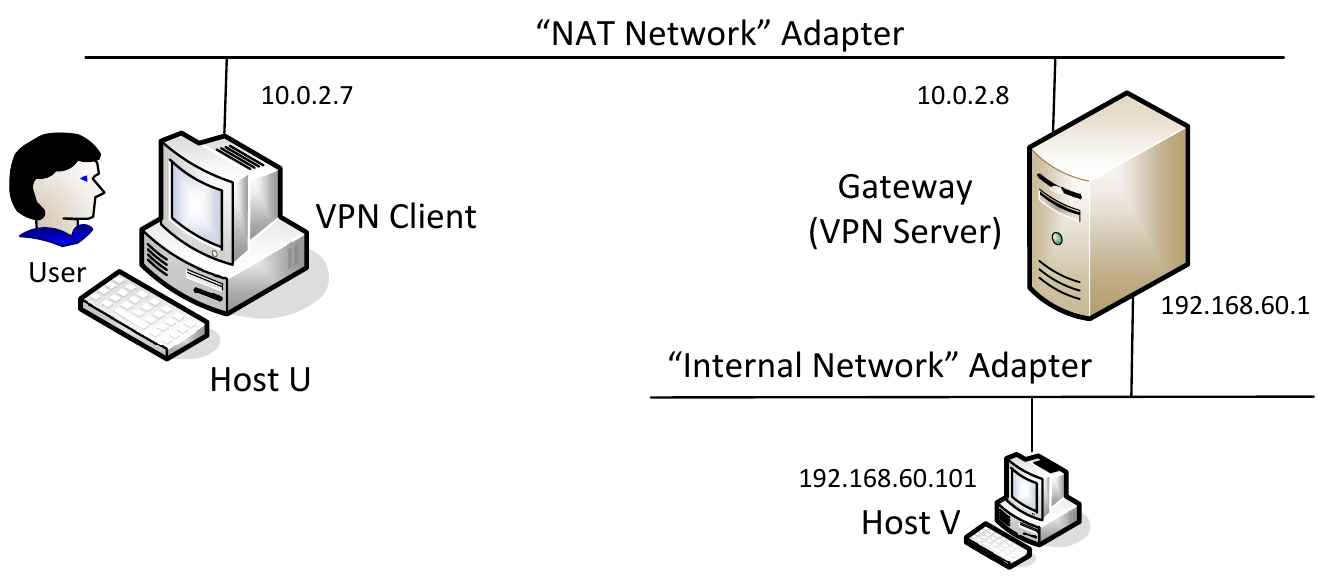
\includegraphics[scale=0.35]{t1_1.png}
    \end{center}{}
    \caption{VM setup for this lab}
    \label{fig:t1_1}
\end{figure}

Figure~\ref{fig:t1_1} shows the network graph of how the VM's should lay out. For redundancy, the IP address table is shown below:

\begin{center}
\begin{tabular}{ |c|c|c| } 
 \hline
 host & IP address(es) \\ 
 \hline
 client & 10.0.2.7  \\ 
 server & 10.0.2.8/192.168.60.1  \\ 
 target & 192.168.60.101 \\
 \hline
\end{tabular}
\end{center}

\subsubsection{Setting up NAT Network}
    The first step to setting up the environment in virtualbox is to set up a NAT Network.
    
    
    \begin{figure}[H]
        \begin{center}
            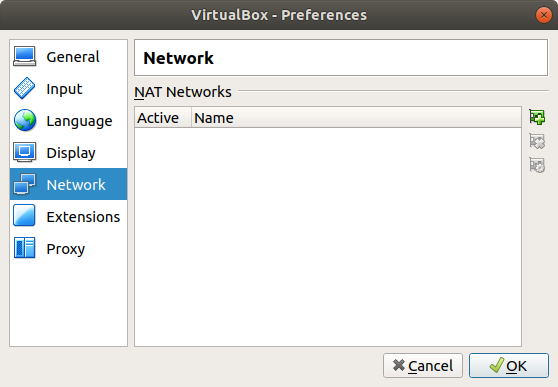
\includegraphics[scale=0.5]{NATNetwork_1.png}
        \end{center}{}
        \caption{VirtualBox Manager Preferences window}
        \label{fig:t1_2}
    \end{figure}
    
    Figure~\ref{fig:t1_2} shows the Virtualbox Manager Preferences window in which the Network tab is selected. Create a new NAT Network by clicking the green plus icon on the top right. 
    
    \begin{figure}[H]
        \begin{center}
            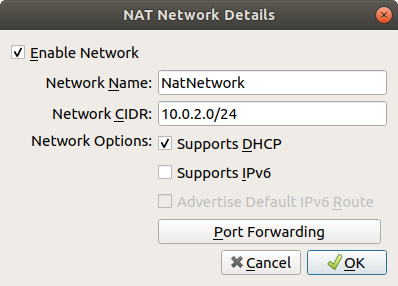
\includegraphics[scale=0.5]{NATNetwork_2.png}
        \end{center}{}
        \caption{Creating new NAT Network}
        \label{fig:t1_3}
    \end{figure}
    
    Figure~\ref{fig:t1_3} shows the window for creating a new NAT Network. Simply keep the defaults as they are and press OK.

\subsubsection{Setting up server settings}
    To set up the server settings through Virtualbox Manager, follow the following steps:
    \begin{enumerate}
        \item open up the settings of the \textbf{server} virtual machine
        \item click \textbf{Network} in the left column
        \item Open \textbf{Adapter 2} tab on the top
        \item create an internal network by changing \textbf{Attached to:} dropdown to \textbf{Internal Network}. Give the internal network a name. We used vpnnet.
    \end{enumerate}
    
    \begin{figure}[H]
        \begin{center}
            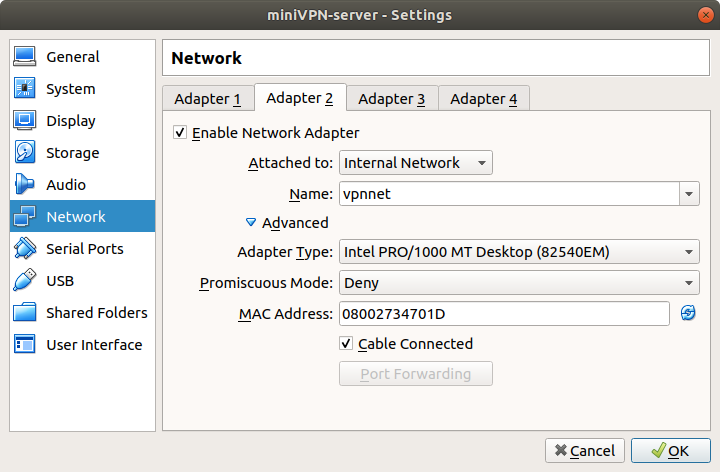
\includegraphics[scale=0.5]{networking_server.png}
        \end{center}{}
        \caption{Server Adapter 2 settings}
        \label{fig:networking_server}
    \end{figure}
    
    Figure~\ref{fig:networking_server} shows the Network settings for the internal network to attach to the target machine. Now we need to set up the public network for the client to access.
    
    \begin{enumerate}
        \item Open \textbf{Adapter 1} tab on the top
        \item Set Adapter 1 to \textbf{Nat Network}, and then choose the NAT Network we created earlier in Figure~\ref{fig:t1_3}
        
    \end{enumerate}
    \begin{figure}[H]
        \begin{center}
            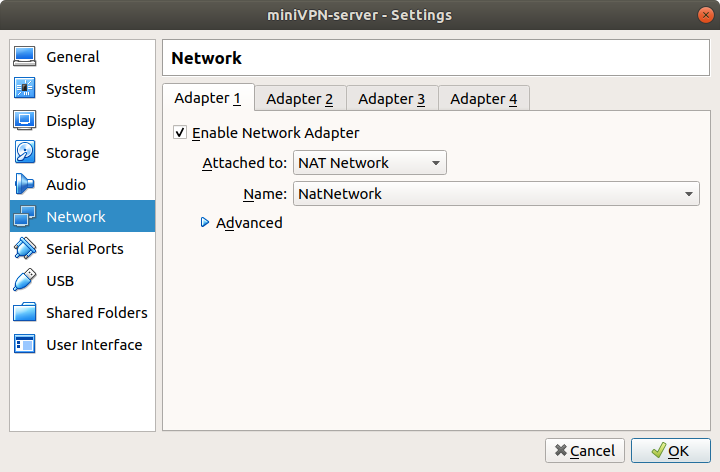
\includegraphics[scale=0.5]{networking_server2.png}
        \end{center}{}
        \caption{Server Adapter 1 settings}
        \label{fig:networking_server_2}
    \end{figure}
    
    Figure~\ref{fig:networking_server_2} shows the network settings for The Adapter 1 for the server. This is the adapter that the client will be accessing as mentioned previously. 

\subsubsection{Setting up target settings}
    \begin{enumerate}
        \item open up the settings of the \textbf{target} virtual machine
        \item click \textbf{Network} in the left column
        \item create an internal network by changing \textbf{Attached to:} dropdown to \textbf{Internal Network}. Give the internal network a name. We used vpnnet.
    \end{enumerate}
    
    \begin{figure}[H]
        \begin{center}
            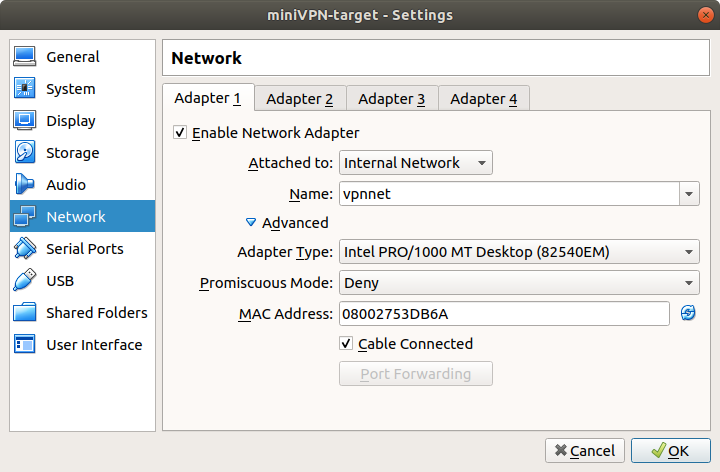
\includegraphics[scale=0.5]{networking_target.png}
        \end{center}{}
        \caption{Server Adapter 2 settings}
        \label{fig:networking_target}
    \end{figure}

\subsubsection{Setting up client settings}
    \begin{enumerate}
        \item open up the settings of the \textbf{client} virtual machine
        \item click \textbf{Network} in the left column
        \item Set Adapter 1 to \textbf{Nat Network}, and then choose the NAT Network we created earlier in Figure~\ref{fig:t1_3}
    \end{enumerate}
    
    \begin{figure}[H]
        \begin{center}
            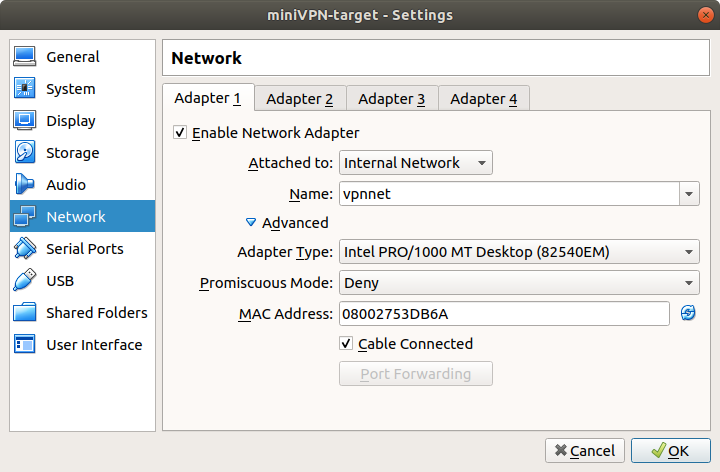
\includegraphics[scale=0.5]{networking_target.png}
        \end{center}{}
        \caption{Server Adapter 2 settings}
        \label{fig:networking_target}
    \end{figure}

\subsubsection{Setting up networking inside the Virtual Machines}

\paragraph{Server}

    Log into your \textbf{server} machine and on the top right click the icon to open the dropdown menu. 
    \begin{figure}[H]
        \begin{center}
            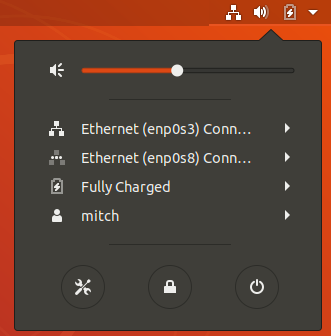
\includegraphics[scale=0.5]{setting_up_server_1.png}
        \end{center}{}
        \caption{Ubuntu 18.04 top right dropdown menu}
        \label{fig:setting_up_server_1}
    \end{figure}
    
    Figure~\ref{fig:setting_up_server_1} shows the drop down menu for Ubuntu 18.04 and two adapters can be seen. enp0s3 is the NAT Network Adapter, whereas enp0s8 is the internal network adapter. Edit the internal network adapter.
    
    \begin{figure}[H]
        \begin{center}
            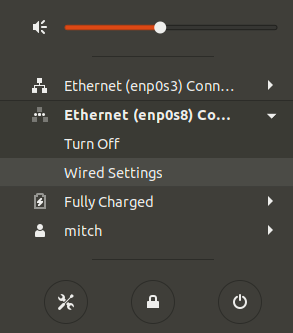
\includegraphics[scale=0.5]{setting_up_server_2.png}
        \end{center}{}
        \caption{Editing Network Adapter Through Menu}
        \label{fig:setting_up_server_2}
    \end{figure}

    Figure~\ref{fig:setting_up_server_2} shows what happens when you expand the network adapter. Simply click Wired Settings now.
    
    \begin{figure}[H]
        \begin{center}
            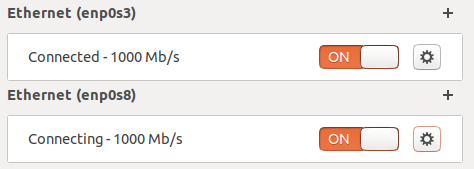
\includegraphics[scale=0.5]{setting_up_server_3.png}
        \end{center}{}
        \caption{Editing Network Adapter Through Menu}
        \label{fig:setting_up_server_3}
    \end{figure}

    You will see Figure~\ref{fig:setting_up_server_3} after clicking Wired Settings, and again, two adapters will be noticed. Click the cog next to the internal network adapter.

    Follow the following guide:
    \begin{enumerate}
        \item Click the \textbf{IPv4} tab
        \item check off \textbf{Manual} in the IPv4 Method section
        \item write the following network settings as shown in Figure~\ref{fig:setting_up_server_4}
    \end{enumerate}

    \begin{figure}[H]
        \begin{center}
            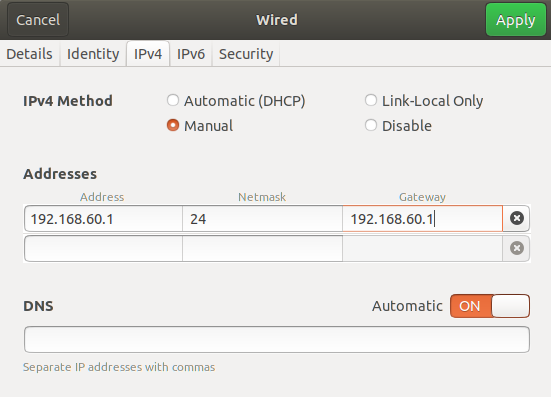
\includegraphics[scale=0.5]{setting_up_server_4.png}
        \end{center}{}
        \caption{Editing Network Adapter Through Menu}
        \label{fig:setting_up_server_4}
    \end{figure}

    Figure~\ref{fig:setting_up_server_4} Shows the final screen for editing the network adapter. Press Apply and then the internal network for the server is set. Now we need to set a static IP address for the public network.
    
    \begin{enumerate}
        \item open a terminal with \textbf{ctrl + alt + t}
        \item edit etc/network/interfaces and add the following
    \end{enumerate}
    
    \begin{verbatim}
    auto enp0s3
    iface enp0s3 inet static
        address 10.0.2.8
        netmask 255.255.255.0
        gateway 10.0.2.1
        dns-nameservers 8.8.8.8 8.8.4.4
    \end{verbatim}
    After adding the static network settings, either restart the system or execute the following:
    \begin{verbatim}
    $ sudo ip a flush enp0s3
    $ sudo systemctl restart networking.service
    \end{verbatim}
    
\paragraph{Target}
    
Similar to the Server, set up the networking as such:
    \begin{figure}[H]
        \begin{center}
            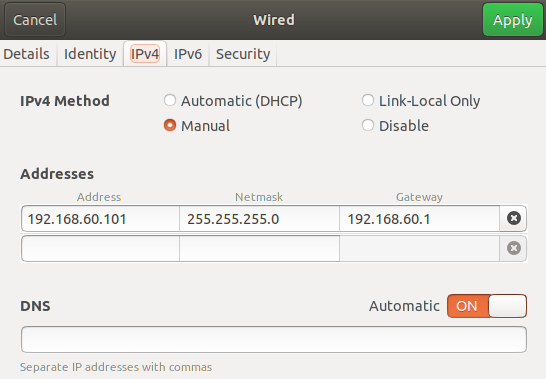
\includegraphics[scale=0.5]{setting_up_target_1.png}
        \end{center}{}
        \caption{target network settings}
        \label{fig:setting_up_target_1}
    \end{figure}


\paragraph{Client}

    Similar to the server, set up the static IP for the NAT Network.

    \begin{enumerate}
        \item open a terminal with \textbf{ctrl + alt + t}
        \item edit /etc/network/interfaces and add the following
    \end{enumerate}
    
    \begin{verbatim}
    auto enp0s3
    iface enp0s3 inet static
        address 10.0.2.7
        netmask 255.255.255.0
        gateway 10.0.2.1
        dns-nameservers 8.8.8.8 8.8.4.4
    \end{verbatim}
    
    An example file is shown below:
    
    \begin{figure}[H]
        \begin{center}
            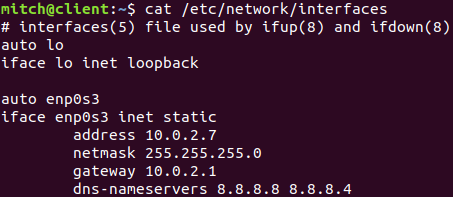
\includegraphics[scale=0.5]{setting_up_client_2.png}
        \end{center}{}
        \caption{example /etc/network/interfaces file}
        \label{fig:setting_up_client_2}
    \end{figure}
    
    
    After adding the static network settings, either restart the system or execute the following:
    \begin{verbatim}
    $ sudo ip a flush enp0s3
    $ sudo systemctl restart networking.service
    \end{verbatim}


\clearpage
\subsection{Task 2: Creating a VPN Tunnel using TUN/TAP}
    Creating a tunnel in this lab setup requires following all of the steps in Task 1. 

    The following section uses code provided by Syracuse University. The code samples can be found here - \url{https://seedsecuritylabs.org/Labs_16.04/Networking/VPN/} And contains source code for the TUN/TAP tunnels.

\subsubsection{setting up Server routing and interfaces}
    On the server, we need to start the vpn server provided by Syracuse University. Run the following command:
    
    \begin{verbatim}
        $ sudo ./vpnserver
    \end{verbatim}
    
    the vpnserver application is a blocking application, so we need to open a new terminal and set up the TUN and permit packet forwarding with:
    
    \begin{verbatim}
        $ sudo ifconfig tun0 192.168.53.1/24 up
        $ sudo sysctl net.ipv4.ip_forward=1
    \end{verbatim}
    
    \begin{figure}[H]
        \begin{center}
            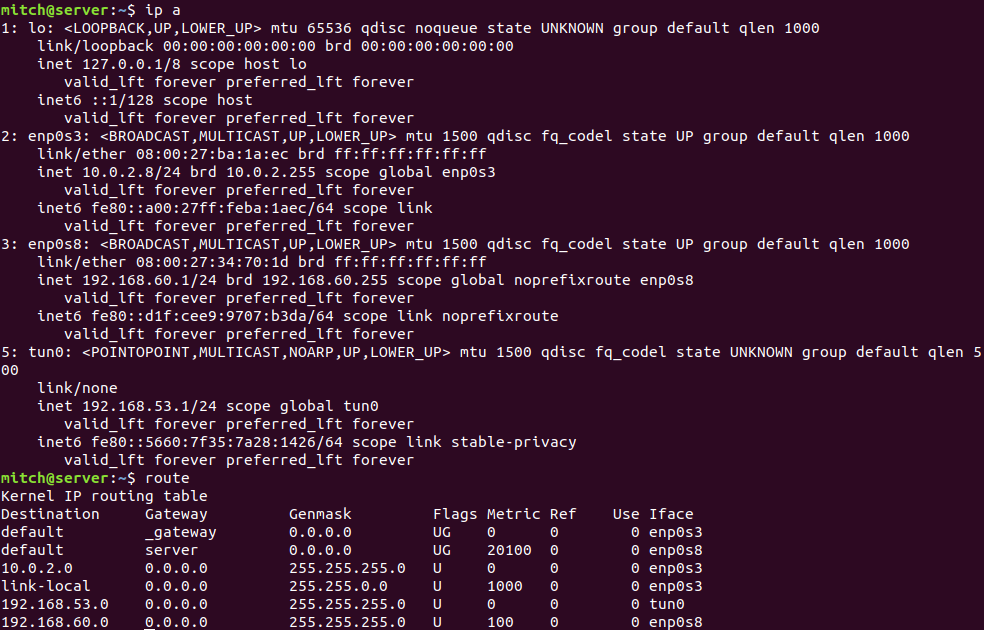
\includegraphics[scale=0.45]{t2_server_routing.png}
        \end{center}{}
        \caption{Task 2 Server Routing and Interfaces}
        \label{fig:t2_server_routing}
    \end{figure}

    Figure~\ref{fig:t2_server_routing} shows the routing and interfaces that the server should show. It can be seen that all 192.168.53.X traffic gets routed to the tun0 interface, whereas all the 192.168.60.X traffic is routed to the enp0s8 interface which is the internal network interface that our target machine is connected to. It can also be seen that tun0 is working and tied to the address 192.168.53.1.

\subsubsection{setting up Client routing and interfaces}
    On the Client, a slight modification to the source code is made. Figure~\ref{fig:t2_modify_vpnclient} shows the change to vpnclient.c which is just a change in one line.
    
    \begin{figure}[H]
        \begin{center}
            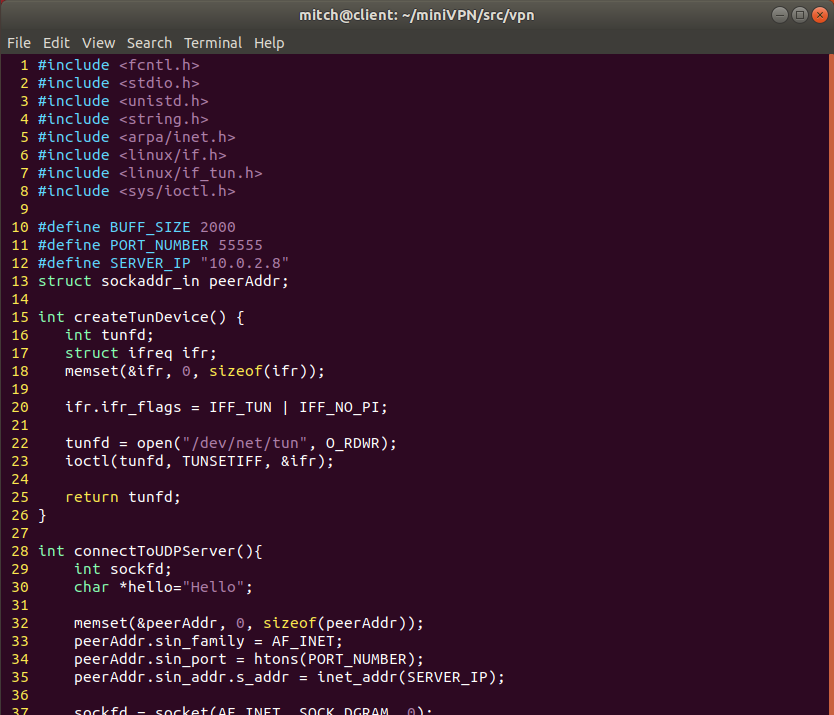
\includegraphics[scale=0.45]{t2_mody_vpnclient.png}
        \end{center}{}
        \caption{Task 2 Modifying vpnclient}
        \label{fig:t2_modify_vpnclient}
    \end{figure}

    \tab In Figure~\ref{fig:t2_modify_vpnclient} it can be seen that line 12 is modified compared to the original source code. The SERVER$\_$IP is hardcoded into the file which we found necessary. When running the progrma while passing through the server IP, the tunnel did not pass through any packets properly.

    After the change in soure code, start the server and create the TUN interface as such:
    \begin{verbatim}
        $ sudo ./vpnclient
    \end{verbatim}
    Just like the server, vpnclient is a blocking application. Therefore, open up a new terminal and set up the interafces as such:
    \begin{verbatim}
        $ sudo ifconfig tun0 192.168.53.5/24 up
        $ sudo route add -net 192.168.60.0/24 tun0
    \end{verbatim}

    \begin{figure}[H]
        \begin{center}
            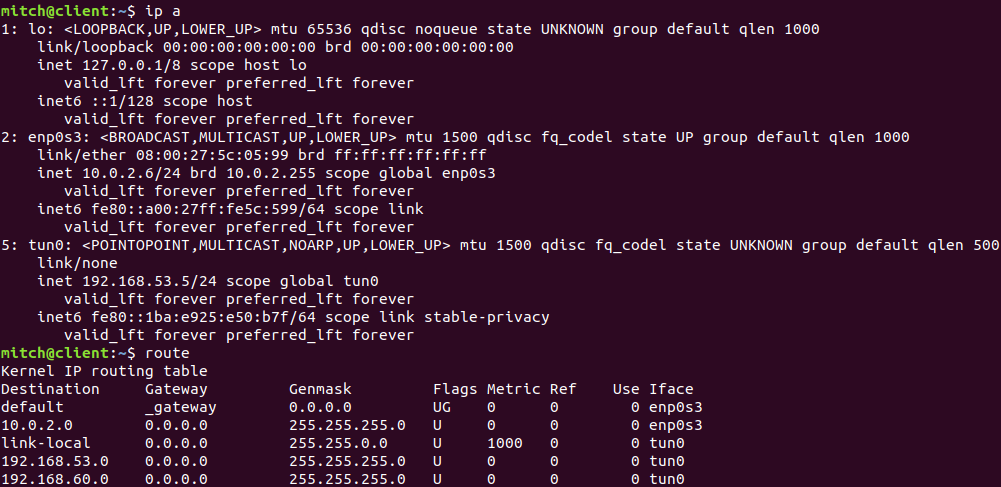
\includegraphics[scale=0.45]{t2_client_routing.png}
        \end{center}{}
        \caption{Task 2 Client Machine Routing and Interfaces}
        \label{fig:t2_client_routing}
    \end{figure}
    
    \tab Figure~\ref{fig:t2_client_routing} shows the routing and network interfaces that the client machine should show. It can be seen all traffic going to 192.168.60.X and 192.168.53.X is being routed to the tun0 interface. It can also be seen that the tun0 interface is linked to the address 192.168.53.5.
    
    
\subsubsection{setting up Target routing and interfaces}
    Setting up the target machine is very simple, it is just adding one route to the routing table. And that route is sending 10.0.2.X traffic back to the server.
    \begin{verbatim}
        $ sudo route add -net 10.0.2.0/24 enp0s3    
    \end{verbatim}

    \begin{figure}[H]
        \begin{center}
            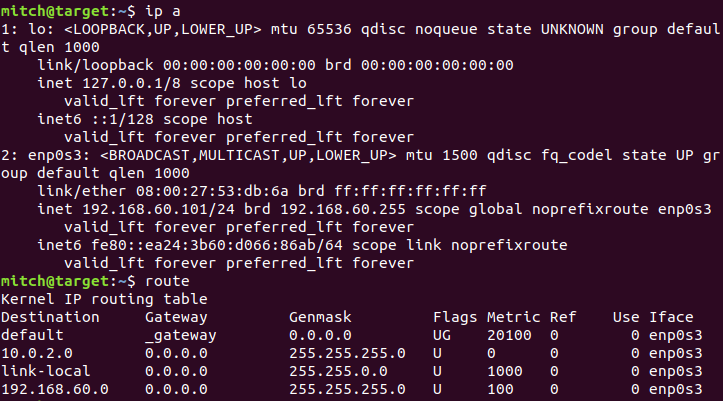
\includegraphics[scale=0.45]{t2_target_routing.png}
        \end{center}{}
        \caption{Task 2 Target Machine Routing and Interfaces}
        \label{fig:t2_target_routing}
    \end{figure}
    
    Figure~\ref{fig:t2_target_routing} shows the routing and network interfaces table. The only addition is adding the 10.0.2.X packets being routed to enp0s3.

\subsubsection{Ping Test}
    We wanted to make sure the ICMP packets from the ping utility command were actually reaching the target. Therefore, we ran the following command on the target:
    \begin{verbatim}
        $ sudo tcpdump ip proto \\icmp
    \end{verbatim}
    The previous command monitors all incoming TCP packets and prints out the icmp packets.

    \begin{figure}[H]
        \begin{center}
            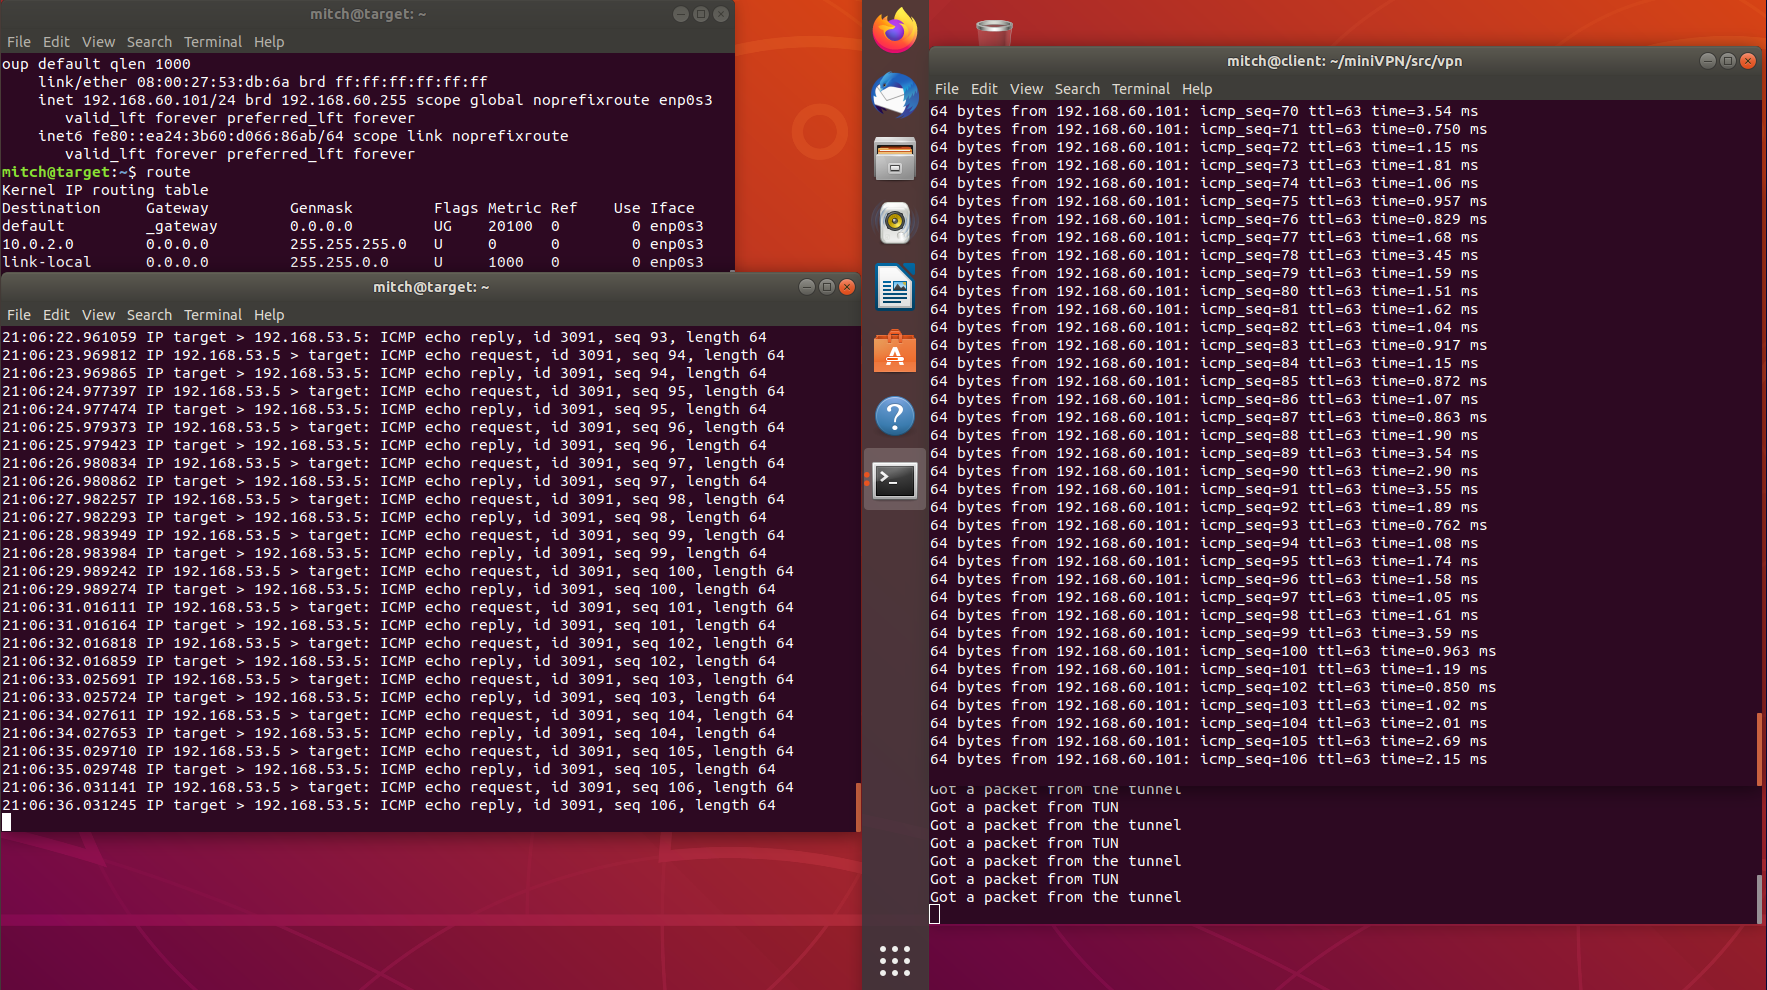
\includegraphics[scale=0.25]{t2_successful_ping.png}
        \end{center}{}
        \caption{Task 2 Client pinging Target}
        \label{fig:t2_successful_ping}
    \end{figure}
    
    Figure~\ref{fig:t2_successful_ping} shows the client machine successfully pinging the target machine. Doing the test is as simple as running the following command on the Client machine:
    
    \begin{verbatim}
        $ ping 192.168.60.101
    \end{verbatim}

    which is successful!
\subsubsection{Tunnel-Breaking Test}
    \tab Due to the fact that our machines are running base Ubuntu 18.04, the telnetd package was needed to be downloaded onto the target machine. After that, we can telnet from the client machine to the target machine with:
    \begin{verbatim}
        $ telnet 192.168.60.101
    \end{verbatim}

    \tab And then make sure that the tunnel is working properly. To do this, we did something simple such as 'touch test1' and verify that the file is created on the target. From there, we break the tunnel with the following command:
    \begin{verbatim}
        sudo ifconfig tun0 down
    \end{verbatim}
    
    Figure~\ref{fig:t2_breaking_tunnel} shows the results of setting the tun0 interface down

    \begin{figure}[H]
        \begin{center}
            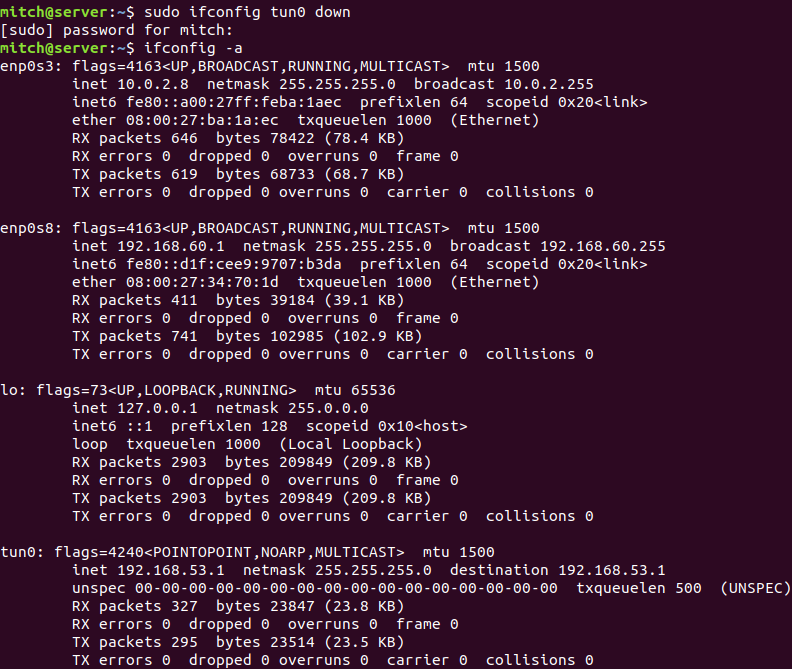
\includegraphics[scale=0.5]{t2_breaking_tunnel.png}
        \end{center}{}
        \caption{Task 2 Breaking VPN Tunnel}
        \label{fig:t2_breaking_tunnel}
    \end{figure}

    Figure~\ref{fig:t2_telnet_tunnel_break} shows the complete flow from initial connection to breaking to reconnection. 

    \begin{figure}[H]
        \begin{center}
            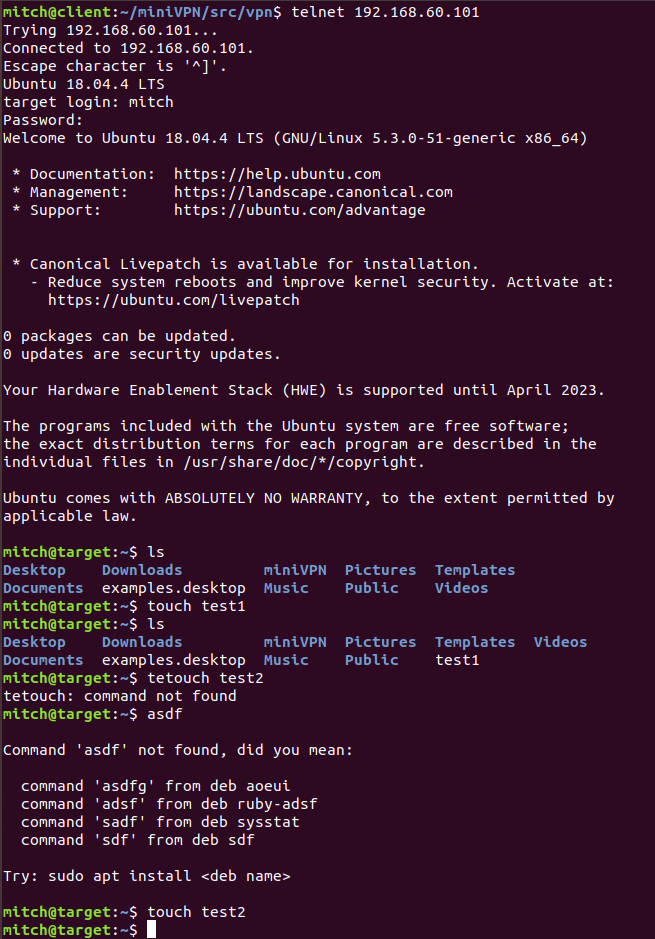
\includegraphics[scale=0.5]{t2_telnet_tunnel_break.png}
        \end{center}{}
        \caption{Task 2 Telnet Tunnel Break Test}
        \label{fig:t2_telnet_tunnel_break}
    \end{figure}

    \tab What was noticed in the lab is that once the tunnel was broken, all keystrokes were frozen in the machine. After reconnecting to the machine, the commands suddenly came back and went through! The commands written during the broken tunnel were 'tetouch test' and 'asdf'. These commands did not show up when written while the tunnel was down, but came back when the tunnel was re-connected. The file test2 was shown on the target machine!

\subsection{Task 3: Set up Routing on Client and Server VMs}

\textit{\item Due to the wrong CA certs shipped with the zip, this task is skipped.}
\subsection{Task 4: Authenticating the VPN Server}
Before a VPN is established, the VPN client must authenticate the VPN server, making sure that the server
is not a fraudulent one. On the other hand, the VPN server must authenticate the client (i.e. user), making
sure that the user has the permission to access the private network. In this task, we implement the server
authentication; the client authentication is in the next task.\\
\tab A typical way to authenticate servers is to use public-key certificates. The VPN server needs to first get
a public-key certificate from a Certificate Authority (CA). When a client makes a connection to the VPN
server, the server will use the certificate to prove it is the intended server. The HTTPS protocol uses this
approach to authenticate web servers, ensuring that you are talking to an intended web server, not a fake
one.\\
\tab In this lab, \emph{MiniVPN} should use such a method to authenticate the VPN server. We can implement
an authentication protocol (such as TLS/SSL) from the scratch, but fortunately, openssl has taken care
most of the work for us. We just need to configure our TLS session properly, so openssl can conduct the
authentication automatically for us.\\
\tab There are three important steps in server authentication: (1) verifying that the server certificate is valid,
(2) verifying that the server is the owner of the certificate, and (3) verifying that the server is the intended
server (for example, if the user intends to visit example.com, we need to ensure that the server is indeed
example.com, not another site). Please point out what lines of the code in your program carry out the
above verifications. In your demonstration, you need to demonstrate two different cases regarding the third
verification: a successful server authentication where the server is the intended server, and a failed server
authentication where the server is not the intended server.\\
\subsubsection{Creating root CA and issuing certs investigations}

This section of this report follows CHAPTER 11. PUBLIC KEY INFRASTRUCTURE from the provided book from class very closely. To complete this task, we need to create our own root CA. Let's start a foundation for creating a CA.

\begin{verbatim}
$ mkdir demoCA
$ cd demoCA
$ mkdir certs crl newcerts
$ touch index.txt serial
$ echo 1000 > serial
$ cd ..
\end{verbatim}

Then we need to create the public/private key pair

\begin{verbatim}
$ openssl req -x509 -newkey rsa:4096 -sha256 -days 3650 \
              -keyout modelCA_key.pem -out modelCA_cert.pem
\end{verbatim}

Now we have modelCA$\_$key.pem and modelCA$\_$cert.pem. Let's generature a publib/private keypair for a website that we will eventualyl call bank32.com

\begin{verbatim}
$ openssl genrsa -aes128 -out bank_key.pem 2048
\end{verbatim}

Now that we have the private key, we need to generate the csr file, or the Certificate Signing Request file.

\begin{verbatim}
$ openssl req -new -key bank_key.pem -out bank.csr -sha256
\end{verbatim}

Now that we have the CSR file for the bank, we can ask the CA to sign the CSR. In this guide, modelCA is our CA.

\begin{verbatim}
$ openssl ca -in bank.csr -out bank_cert.pem -md sha256 \
             -cert modelCA_cert.pem -keyfile modelCA_key.pem 
             -config openssl.cnf
\end{verbatim}

\tab The above command does quite a bit. It uses the CSR file from the bank, and uses the certificate and private key of the CA to sign the cert. This will generate bank$\_$cert.pem.

\tab Now that we have the private key and cert for the fake bank website, we can run a server with openssl with the following command:

\begin{verbatim}
mitch@server:~/miniVPN/src/tls/cert_server$ openssl s_server \
                                        -cert bank_all.pem -accept 4433 -www
\end{verbatim}

Now if we put the following line into /etc/hosts:
\begin{verbatim}
127.0.0.1	bank32.com
\end{verbatim}
We can access the server with 
\begin{verbatim}
$ openssl s_client -connect bank32.com:4433 -CAfile modelCA_cert.pem
\end{verbatim}
\tab This was all done on the server VM, but we want to connect to the server VM from the client VM. To deviate from the guide a little bit, we attempt to establish a connection from the client. On the client machine we add the following to /etc/hosts:
\begin{verbatim}
10.0.2.8      dzurick.com
\end{verbatim}

and we copy the modelCA$\_$cert.pem file to the client, we can access the server remotely! Success.
    \begin{figure}[H]
        \begin{center}
            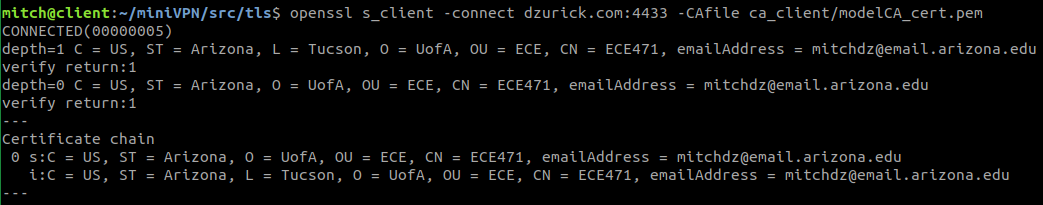
\includegraphics[scale=0.6]{t4_2.png}
        \end{center}{}
        \caption{Connecting to Server from Client with CA's cert}
        \label{fig:t4_2}
    \end{figure}

\tab Figure~\ref{fig:t4_2} shows the results from trying to access our fake website dzurick.com which is 'hosted' on our remote server with a certificate. Let's try that again without the certificate and see what happens. Do note the terminal now has a black background because I decided to change my terminal to terminator halfway through :).

    \begin{figure}[H]
        \begin{center}
            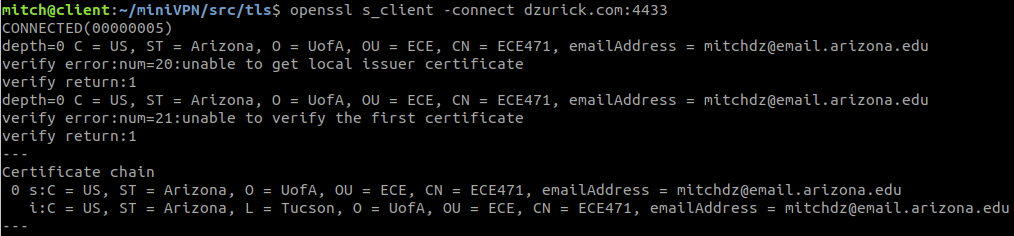
\includegraphics[scale=0.6]{t4_3.png}
        \end{center}{}
        \caption{Connecting to Server from Client without CA's cert}
        \label{fig:t4_3}
    \end{figure}
    
\tab Figure~\ref{fig:t4_3} shows what happens when we do not use the cert file. We can see that the response says "Unable to get local issuer certificate".

\tab Now just for fun, let's see what happens when we try to connect to the server but purposely close the server. Simply running 'ctrl + c' on the server to kill the process and then attempting a connection via the client again.

    \begin{figure}[H]
        \begin{center}
            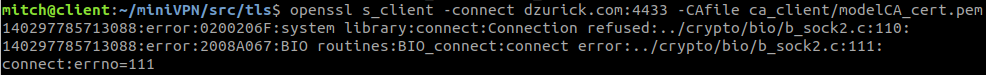
\includegraphics[scale=0.6]{t4_connect_no_server_up.PNG}
        \end{center}{}
        \caption{Connecting to Server from Client without CA's cert}
        \label{fig:t4_connect_no_server_up}
    \end{figure}

\tab Figure~\ref{fig:t4_connect_no_server_up} shows the results of trying to connect. That's about what we expected! Now to access the server through the web browser, we need Firefox to accept the CA that we created.

    \begin{figure}[H]
        \begin{center}
            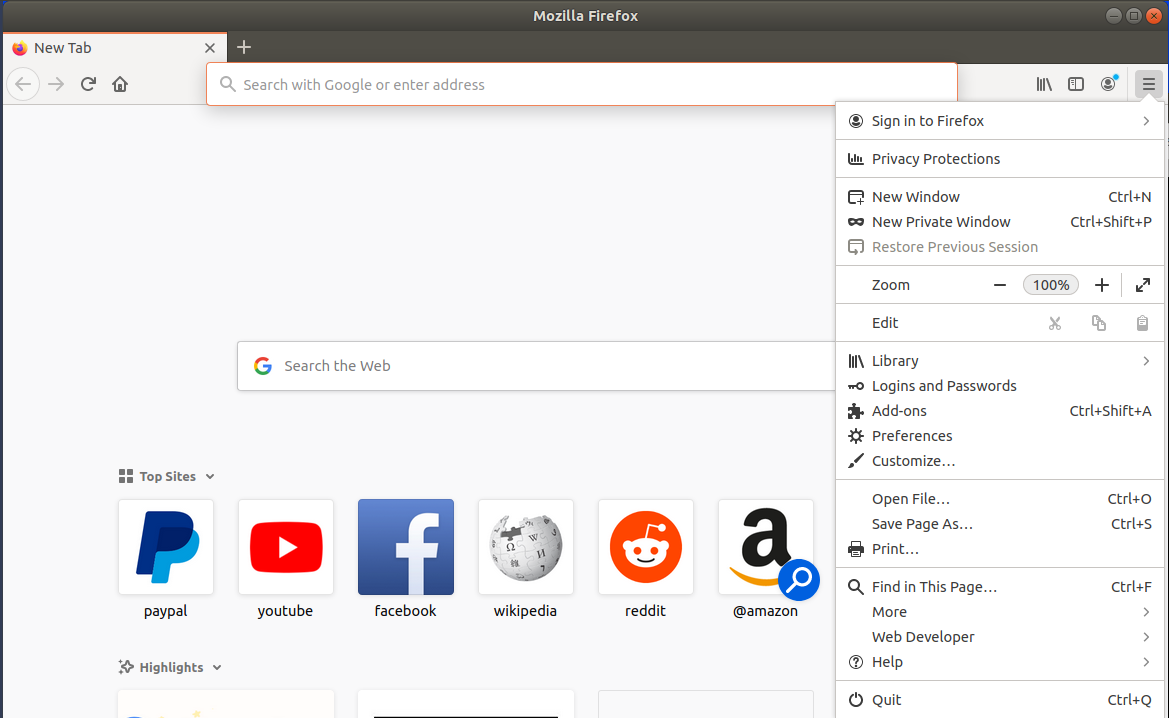
\includegraphics[scale=0.5]{t4_4.png}
        \end{center}{}
        \caption{Firefox on the server VM}
        \label{fig:t4_4}
    \end{figure}

\tab To access the Firefox settings, first click to hamburger icon on the top right as shown in Figure~\ref{fig:t4_4} and then click 'Preferences'.

    \begin{figure}[H]
        \begin{center}
            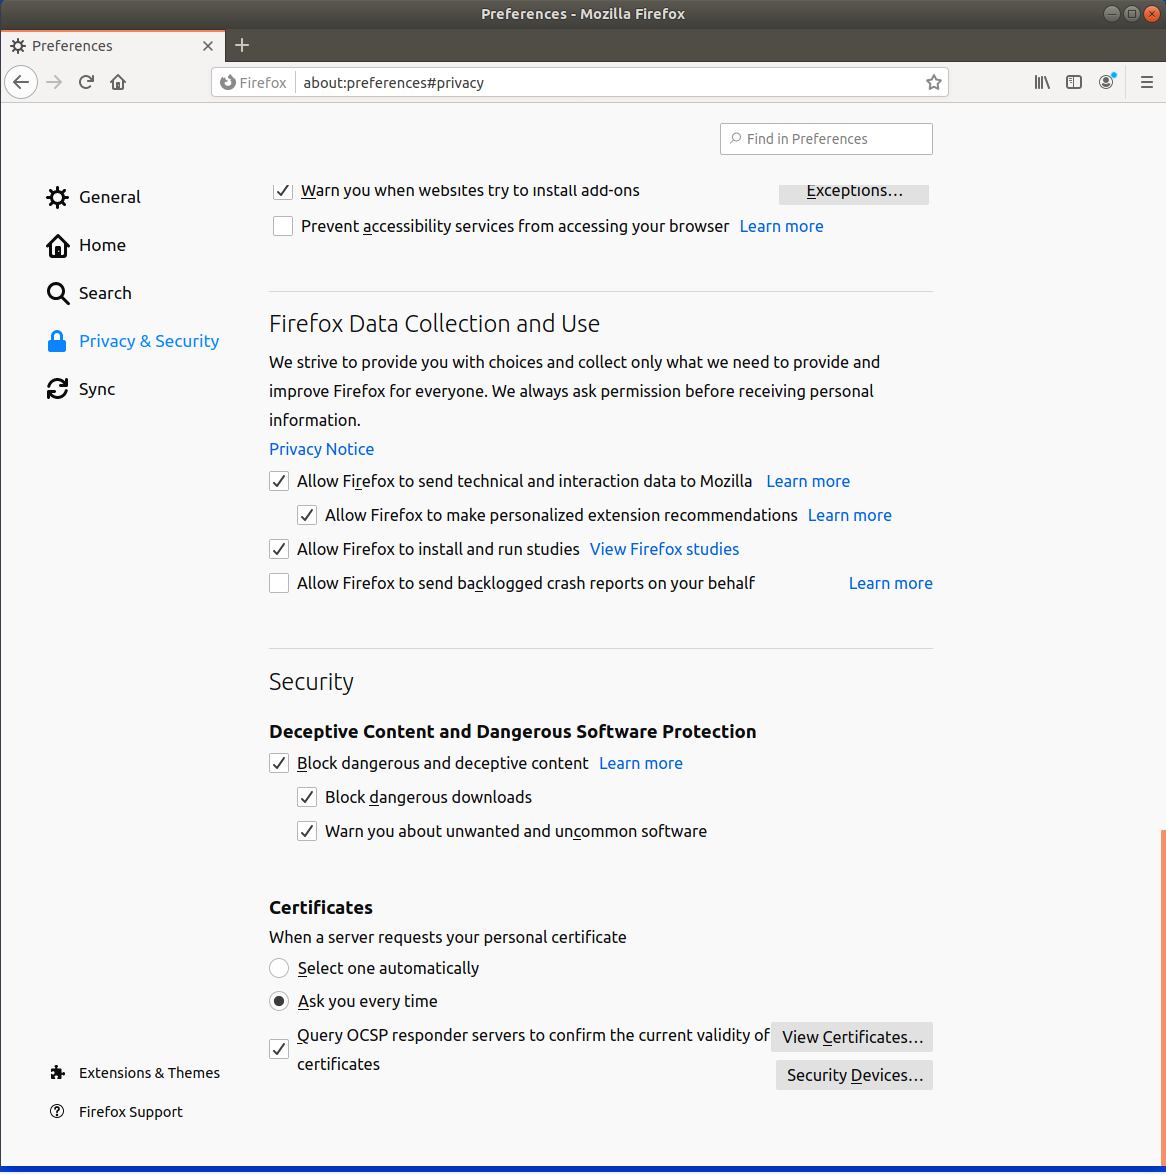
\includegraphics[scale=0.5]{t4_5.png}
        \end{center}{}
        \caption{Firefox Certificates settings}
        \label{fig:t4_5}
    \end{figure}

To view Certificates in Firefox, click 'Privacy & Security' on the left tab, and scroll all the way down to 'Security' as shown in Figure~\ref{fig:t4_5}.
    
    \begin{figure}[H]
        \begin{center}
            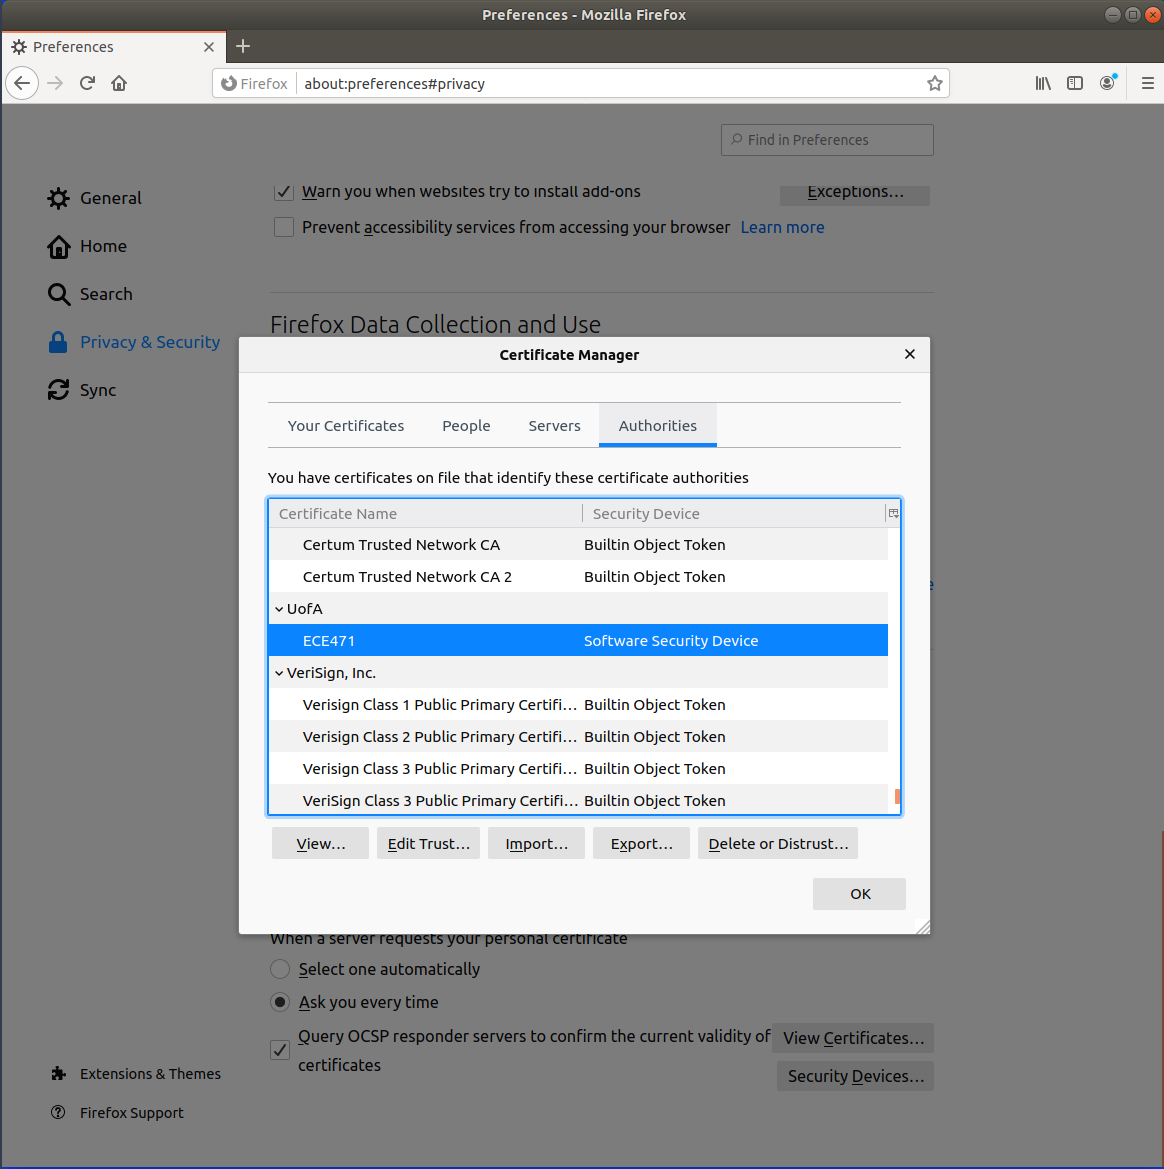
\includegraphics[scale=0.5]{t4_6.png}
        \end{center}{}
        \caption{selecting our modelCA cert}
        \label{fig:t4_6}
    \end{figure}
    
If not already added, you can click 'Import...' in Figure~\ref{fig:t4_6}, but the cert was already added. We can view the certificate by clicking 'View...'
    
    
    \begin{figure}[H]
        \begin{center}
            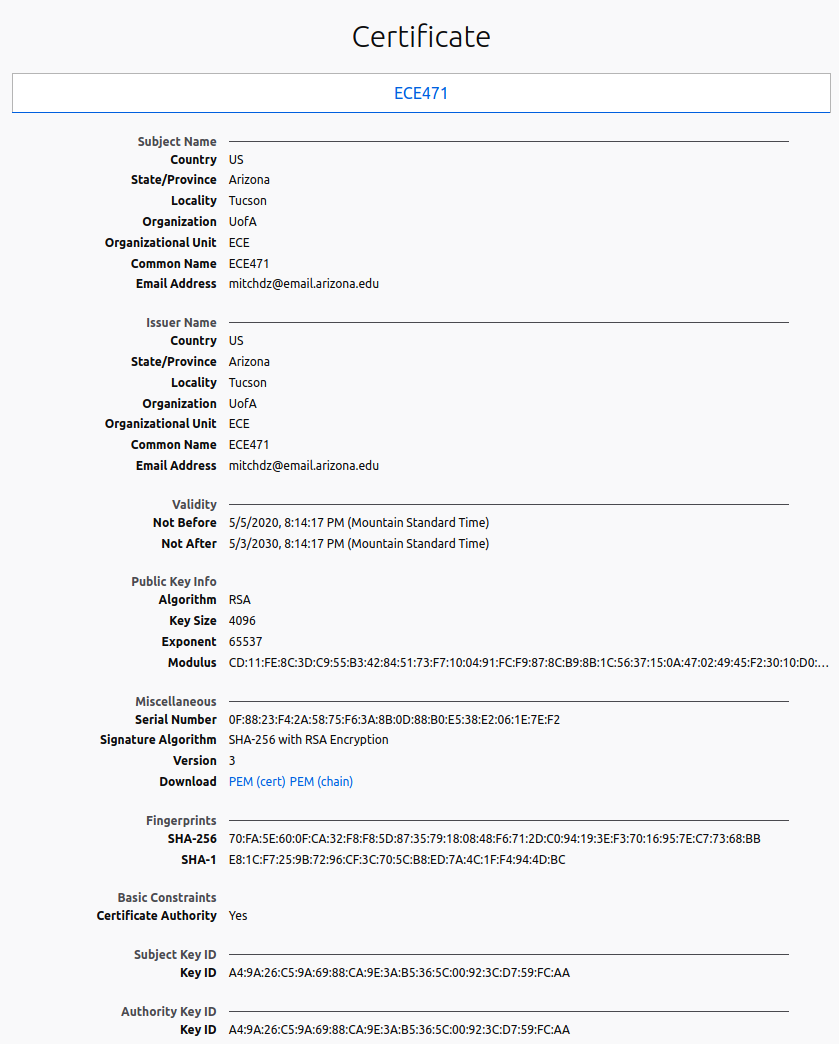
\includegraphics[scale=0.5]{t4_7.png}
        \end{center}{}
        \caption{Viewing our modelCA cert}
        \label{fig:t4_7}
    \end{figure}

Figure~\ref{fig:t4_7} shows the details of our certificate inside Firefox. The issuer name and subject name are things that I filled out when creating the cert. I had no idea what I was doing, so I made my organization UofA, Org unit ECE, and common name ECE471.


\subsubsection{Three Important Steps in Server Authentication}
As mentioned before, there are three important steps in server authentication. The below sections cover each three important steps. When we contact the server we get the following response back:

With the \texttt{lstlisting} environment and \texttt{breaklines=true}:
\begin{lstlisting}
mitch@client:~/miniVPN/src/tls$ openssl s_client -connect dzurick.com:4433 -CAfile ca_client/modelCA_cert.pem 
CONNECTED(00000005)
depth=1 C = US, ST = Arizona, L = Tucson, O = UofA, OU = ECE, CN = ECE471, emailAddress = mitchdz@email.arizona.edu
verify return:1
depth=0 C = US, ST = Arizona, O = UofA, OU = ECE, CN = ECE471, emailAddress = mitchdz@email.arizona.edu
verify return:1
---
Certificate chain
 0 s:C = US, ST = Arizona, O = UofA, OU = ECE, CN = ECE471, emailAddress = mitchdz@email.arizona.edu
   i:C = US, ST = Arizona, L = Tucson, O = UofA, OU = ECE, CN = ECE471, emailAddress = mitchdz@email.arizona.edu
---
Server certificate
-----BEGIN CERTIFICATE-----
MIIE9zCCAt+gAwIBAgICEAIwDQYJKoZIhvcNAQELBQAwgYgxCzAJBgNVBAYTAlVT
MRAwDgYDVQQIDAdBcml6b25hMQ8wDQYDVQQHDAZUdWNzb24xDTALBgNVBAoMBFVv
ZkExDDAKBgNVBAsMA0VDRTEPMA0GA1UEAwwGRUNFNDcxMSgwJgYJKoZIhvcNAQkB
FhltaXRjaGR6QGVtYWlsLmFyaXpvbmEuZWR1MB4XDTIwMDUwNjE3MzgxNVoXDTIx
MDUwNjE3MzgxNVowdzELMAkGA1UEBhMCVVMxEDAOBgNVBAgMB0FyaXpvbmExDTAL
BgNVBAoMBFVvZkExDDAKBgNVBAsMA0VDRTEPMA0GA1UEAwwGRUNFNDcxMSgwJgYJ
KoZIhvcNAQkBFhltaXRjaGR6QGVtYWlsLmFyaXpvbmEuZWR1MIIBIjANBgkqhkiG
9w0BAQEFAAOCAQ8AMIIBCgKCAQEAvWIpO9Di7nF4eiJ/+AFCS2weDb3zqTmxMw4d
2sjucDzp1U4g9Vf3EhNrIwxymK/l1y54tw9//sv8YorsbwvBm2NJzYMq83Tif2Up
F3C+vABfOcy4fQSd0C3YlekWHORc8oHpU+E4UzrpBmMLnK/0yIGXusUsPyv3zOLt
24NxEAe0Uob1wYJiDtGG0JNQ8GicbVkaJJtBxFmJ9UXglbQBY78mmRo+NoeYnD2v
0HQpbI35QcvACJH8Kjc8cRfHv3saOnVPW6dXPffGS9HO3WlYvm7WzLMoWaDA0PL3
wKc1VU/+Z2sI3oYDx9QBemhzLQkDEyPaD3SDhbZkFgy3IcM37wIDAQABo3sweTAJ
BgNVHRMEAjAAMCwGCWCGSAGG+EIBDQQfFh1PcGVuU1NMIEdlbmVyYXRlZCBDZXJ0
aWZpY2F0ZTAdBgNVHQ4EFgQU8hFJX/ANLxE5cIifD0mNklM/QCgwHwYDVR0jBBgw
FoAUpJomxZppiMqeOrU2XACSPNdZ/KowDQYJKoZIhvcNAQELBQADggIBAGqizidD
zkhXVvCxoClyRnXkCGxGFA+5lDGWHMw1dRwuduKpOlEYT2Ahfi3saIpG3NrkIhzX
pLRQ92JEHvW76wtE2hRHc8NWuiBCo72paZoS4IqLUl9w5WLC+bdfpjQI3Kz4Ehtl
wAjCGmWfZWy/+WRTRqxWqMD4i4Vfhu8oBN4+QymCXTJIOQs1HK7lp4cQf77lVWAY
jx7kQZqWhCCK6BX3lAlDmX+akY7uOXbZTIwUMoTWFheoreOuoDxNawrFcJDR25J5
9cEtnhCH6HG1/tsa1OhFey0b58Ij0RCMMlf3isX8bSAKaV5whoigkUlA2zvWnt1P
cAN7Ome0s8439Xuik7z0BUzYksLKfqmsHQSGR0vvlIanJw4FK4qxgseBi4pF/3mb
NESQIo1tY/LK3ewSMexO9LzdClqBFt7ZnMjmn3eaM9dp+O76A+e28BwbaOizM8Lp
1aSd82vIikLoQOZhwNC9VhxLkCG/6u94ZQLVOYA7r8KUazwdglnpaWXyqOZHnAN1
c0jus6YD9JxXW3NreVV5EN8SKKH/WXW2FkZQetBr//uBvvhDE93LWCs3ZpqJI1tN
hoYrRW+c+vTSjJTvqsJdchMctBH3gnm4VfjrKey9aFJzMjETYDLyBU3GAQ7r6YAS
F1w+HXCOUG5OVWu3Y8MuzrCxU+Spb3z6pnxO
-----END CERTIFICATE-----
subject=C = US, ST = Arizona, O = UofA, OU = ECE, CN = ECE471, emailAddress = mitchdz@email.arizona.edu

issuer=C = US, ST = Arizona, L = Tucson, O = UofA, OU = ECE, CN = ECE471, emailAddress = mitchdz@email.arizona.edu

---
No client certificate CA names sent
Peer signing digest: SHA256
Peer signature type: RSA-PSS
Server Temp Key: X25519, 253 bits
---
SSL handshake has read 1831 bytes and written 393 bytes
Verification: OK
---
New, TLSv1.3, Cipher is TLS_AES_256_GCM_SHA384
Server public key is 2048 bit
Secure Renegotiation IS NOT supported
Compression: NONE
Expansion: NONE
No ALPN negotiated
Early data was not sent
Verify return code: 0 (ok)
---
---
Post-Handshake New Session Ticket arrived:
SSL-Session:
    Protocol  : TLSv1.3
    Cipher    : TLS_AES_256_GCM_SHA384
    Session-ID: CCF35EB20153A747B6F3913BCD3A1A7218561F3CC633DA2A6F2893C70A580D81
    Session-ID-ctx: 
    Resumption PSK: 7BF728E86E9950FD428AC4DD8367E98F182BAE257D3FC863B3B7D1301F4A4EB4D5741B771D6F1B39DF9363FB75A482F1
    PSK identity: None
    PSK identity hint: None
    SRP username: None
    TLS session ticket lifetime hint: 7200 (seconds)
    TLS session ticket:
    0000 - d4 cb b7 5e 11 13 ed 64-70 23 45 80 9b 80 fc c5   ...^...dp#E.....
    0010 - 98 c1 ce 0e 93 89 59 4f-c2 9b d0 a6 45 45 6d 4e   ......YO....EEmN
    0020 - e1 d8 19 8a 5d 28 cc b6-78 a2 e9 07 c1 c5 38 56   ....](..x.....8V
    0030 - 5b 2a 06 43 63 55 3a 14-56 64 ae 4a f6 00 69 6d   [*.CcU:.Vd.J..im
    0040 - 7c aa 3a 85 3f 4e 49 c0-1b 9a dd 98 d9 51 df 8f   |.:.?NI......Q..
    0050 - f7 cf 5e 7c e8 9f 19 c8-69 9a b9 0a c4 d3 d7 d9   ..^|....i.......
    0060 - c3 f8 4c 14 a9 76 c2 c1-d1 5a f8 2b da 70 96 71   ..L..v...Z.+.p.q
    0070 - 19 bc 65 02 e9 49 6e 34-29 a0 d5 48 c4 a9 3b 16   ..e..In4)..H..;.
    0080 - 33 70 36 99 f3 04 91 8c-be 7a 15 08 b5 35 a9 3d   3p6......z...5.=
    0090 - 0f 1c 1f 85 ee 39 9e c4-1c 94 e2 aa f1 c0 fb f5   .....9..........
    00a0 - 51 79 01 fa bd ba a8 12-40 cf 5d 73 c4 8d 40 82   Qy......@.]s..@.
    00b0 - 24 88 b0 43 d3 4a 79 5e-ca fb eb 72 e7 a0 78 60   $..C.Jy^...r..x`

    Start Time: 1588787865
    Timeout   : 7200 (sec)
    Verify return code: 0 (ok)
    Extended master secret: no
    Max Early Data: 0
---
read R BLOCK
---
Post-Handshake New Session Ticket arrived:
SSL-Session:
    Protocol  : TLSv1.3
    Cipher    : TLS_AES_256_GCM_SHA384
    Session-ID: 7248390A7EF8898CD463306559ACF495CEBCC3E4C4564F6727DFE604690569C4
    Session-ID-ctx: 
    Resumption PSK: 708857341E4A4EEF4B624A2C93F6665E6698F681876DBCB0E414642AEB9ECAE6653EC6F9F72238AF20F52ECC997A598D
    PSK identity: None
    PSK identity hint: None
    SRP username: None
    TLS session ticket lifetime hint: 7200 (seconds)
    TLS session ticket:
    0000 - d4 cb b7 5e 11 13 ed 64-70 23 45 80 9b 80 fc c5   ...^...dp#E.....
    0010 - 4e 2b fb 1e 68 89 7b f6-e8 de 54 7c a2 bd 6e 89   N+..h.{...T|..n.
    0020 - f5 99 fa 51 00 e1 71 fc-98 4f 8f 0c 74 79 72 4a   ...Q..q..O..tyrJ
    0030 - 7e a2 8c ce 4b 44 09 45-41 2b 73 51 53 55 9d 35   ~...KD.EA+sQSU.5
    0040 - 95 ed 00 d9 be a0 74 63-7f c8 2f e4 32 ab 73 3b   ......tc../.2.s;
    0050 - c7 16 ec f0 82 49 e9 05-8a c1 c4 ef 58 09 7a ed   .....I......X.z.
    0060 - 37 ca 4d b1 29 01 9e 5d-46 9b 8c 44 c3 67 95 1a   7.M.)..]F..D.g..
    0070 - b1 60 85 c9 c6 ba 42 80-00 a5 1f 54 f4 7c ad f1   .`....B....T.|..
    0080 - 4f e5 72 25 61 b5 58 eb-06 47 ee 9c b7 3f 8c 6c   O.r%a.X..G...?.l
    0090 - 74 e7 2c 58 99 31 74 dd-05 3e 9d ef 8d 84 0b 43   t.,X.1t..>.....C
    00a0 - cc f1 48 69 87 28 d5 e7-21 88 00 d8 9b a7 13 e1   ..Hi.(..!.......
    00b0 - 70 d8 50 59 58 cf ec da-c3 62 b1 6c 8d 71 83 60   p.PYX....b.l.q.`

    Start Time: 1588787865
    Timeout   : 7200 (sec)
    Verify return code: 0 (ok)
    Extended master secret: no
    Max Early Data: 0
---
read R BLOCK
    \end{lstlisting}
\paragraph{verifying that the server certificate is valid}
Like all of these verifications, there is a trust that the CA is a trustworthy source. The line of code that proves the validity is when the CA signs the certificate with the following line:
\begin{verbatim}
$ openssl ca -in bank.csr -out bank_cert.pem -md sha256\
 -cert modelCA_cert.pem -keyfile modelCA_key.pem
\end{verbatim}
The bank$\_$cert.pem file that is generated is verified via the CA.

\paragraph{verifying that the server is the owner of the certificate}
Similar to the previous command, the generated certificate has information about the server. The certificate has a private key in it that only the owning server should have access to.
\paragraph{verifying that the server is the intended server}
The server has a certificate that the CA trusts, and you trust the CA as well. This trust verifies that the server is the intended server.

\subsection{Task 5: Authenticating the VPN Client}
Accessing the machines inside a private network is a privilege that is only granted to authorized users, not to everybody. Therefore, only authorized users are allowed to establish a VPN tunnel with the VPN server. In this task, authorized users are those who have a valid account on the VPN server. We will therefore use the standard password authentication to authenticate users. Basically, when a user tries to establish a VPN tunnel with the VPN server, the user will be asked to provide a user name and a password. The server will check its shadow file (/etc/shadow); if a matching record is found, the user is authenticated, and the VPN tunnel will be established. If there is no match, the server will break its connection with the user, and thus no tunnel will be established.

The following program shows how to authenticate a user using the account information stored in the shadow
file. The program uses getspnam() to get a given user’s account information from the shadow file,
including the hashed password. It then uses crypt() to hash a given password and see whether the result
matches with the values fetched from the shadow file. If so, the user name and the password match, and the
authentication is successful.

\begin{verbatim}
#include <stdio.h>
#include <string.h>
#include <shadow.h>
#include <crypt.h>
int login(char *user, char *passwd)
{
struct spwd *pw;
char *epasswd;
pw = getspnam(user);
if (pw == NULL) {
return -1;
}
printf("Login name: %s\n", pw->sp_namp);
printf("Passwd : %s\n", pw->sp_pwdp);
epasswd = crypt(passwd, pw->sp_pwdp);
if (strcmp(epasswd, pw->sp_pwdp)) {
return -1;
}
return 1;
}
void main(int argc, char** argv)
{
if (argc < 3) {
printf("Please provide a user name and a password\n");
return;
}
int r = login(argv[1], argv[2]);
printf("Result: %d\n", r);
}
\end{verbatim}

We can compile the code above and run it with a user name and a password. It should be noted that the
root privilege is needed when reading from the shadow file. See the following commands for compilation
and execution.

\begin{verbatim}
$ gcc login.c -lcrypt
$ sudo ./a.out seed dees
\end{verbatim}

It should be noted that we use -lcrypt in the above compilation; we used -lcrypto when compiling
our TLS programs. The crypt and crypto are two different libraries, so this is not a typo. Let's test this program.

    \begin{figure}[H]
        \begin{center}
            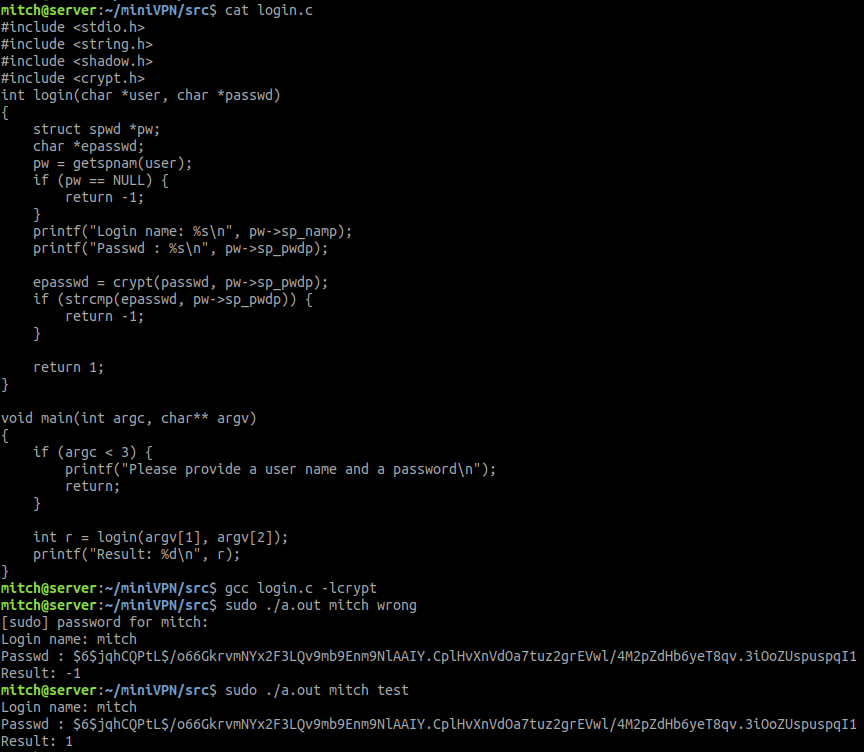
\includegraphics[scale=0.6]{t5_1.PNG}
        \end{center}{}
        \caption{Task 5: Testing Accessing the Shadow File}
        \label{fig:t5_1}
    \end{figure}

Figure~\ref{fig:t5_1} shows the results of compiling and running the program. My use has a username of "mitch" and a password of "test". It can be seen that when given the wrong password, that the program returns an error. Let's integrate this into the tlsserver. The integration was made on a copy of the tls folder provided by SEED Labs, and my folder can be found \href{https://github.com/mitchdz/miniVPN/tree/master/src/mytls}{here}.

The main function for the client stays mostly the same with a few additions.

\begin{verbatim}
int main(int argc, char *argv[])
{
   char *hostname = "yahoo.com";
   int port = 443;

   char *user = "USERNAME";
   char *pass = "PASSWORD";

   if (argc > 1) hostname = argv[1];
   if (argc > 2) port = atoi(argv[2]);
   if (argc > 3) user = argv[3];
   if (argc > 4) pass = argv[4];


   /*----------------TLS initialization ----------------*/
   SSL *ssl   = setupTLSClient(hostname);

   /*----------------Create a TCP connection ---------------*/
   int sockfd = setupTCPClient(hostname, port);

   /*----------------TLS handshake ---------------------*/
   SSL_set_fd(ssl, sockfd);
   int err = SSL_connect(ssl); CHK_SSL(err);
   printf("SSL connection is successful\n");
   printf ("SSL connection using %s\n", SSL_get_cipher(ssl));

   /*----------------Send/Receive data --------------------*/
   char buf[9000];
   char sendBuf[200];
   sprintf(sendBuf, "GET / HTTP/1.1\n
      Host: %s\n\
      User: %s\n\
      Pass: %s\n", hostname, user, pass);
   SSL_write(ssl, sendBuf, strlen(sendBuf));

   int len;
   do {
     len = SSL_read (ssl, buf, sizeof(buf) - 1);
     buf[len] = '\0';
     printf("%s\n",buf);
   } while (len > 0);
}
\end{verbatim}

The addition here is that there are two more input arguments. In addition to the hostname and port, a username and password is expected. Therefore, instead of running the command `./tlsclient dzurick.com 4433` it would be `./tlsclient dzurick.com 4433 mitch test`, where mitch is the username, and test is the password. These variables are then sent through SSL. The message sent through the tunnel looks like the below sample.

\begin{verbatim}
GET / HTTP/1.1
Host: dzurick.com
User: mitch
Pass: test
\end{verbatim}

Which the server will parse.

The server code for processing a request is as follows:


\begin{verbatim}
<code snipped>
  6 #include <stdio.h>
  7 #include <string.h>
  8 #include <shadow.h>
  9 #include <crypt.h>
 10 
 11 #define MAXSIZE 50
<code snipped>
 84 int login(char *user, char *passwd)
 85 {
 86     struct spwd *pw;
 87     char *epasswd;
 88     pw = getspnam(user);
 89     if (pw == NULL) {
 90         return -1;
 91     }
 92     printf("Login name: %s\n", pw->sp_namp);
 93     printf("Passwd : %s\n", pw->sp_pwdp);
 94 
 95     epasswd = crypt(passwd, pw->sp_pwdp);
 96     if (strcmp(epasswd, pw->sp_pwdp)) {
 97         return -1;
 98     }
 99 
100     return 1;
101 }
102 
103 
104 void processRequest(SSL* ssl, int sock)
105 {
106     char buf[1024];
107     int len = SSL_read (ssl, buf, sizeof(buf) - 1);
108 
109     char inHost[MAXSIZE], inUser[MAXSIZE], inPass[MAXSIZE];
110     sscanf(buf, "GET / HTTP/1.1\n\
111       Host: %s\n\
112       User: %s\n\
113       Pass: %s"\
114       , inHost, inUser, inPass);
115 
116     if (login(inUser, inPass) == -1) return 0;
117 
118     buf[len] = '\0';
119     printf("Received: %s\n",buf);
120 
121 
122     // Construct and send the HTML page
123     char *html =
124         "HTTP/1.1 200 OK\r\n"
125         "Content-Type: text/html\r\n\r\n"
126         "<!DOCTYPE html><html>"
127         "<head><title>Hello World</title></head>"
128         "<style>body {background-color: black}"
129         "h1 {font-size:3cm; text-align: center; color: white;"
130         "text-shadow: 0 0 3mm yellow}</style></head>"
131         "<body><h1>Hello, world!</h1></body></html>";
132     SSL_write(ssl, html, strlen(html));
133     SSL_shutdown(ssl);  SSL_free(ssl);
134 }

\end{verbatim}

In the above server code, line numbers are provided so I can more easily point to what has changed. Lines 6-11 are added includes for accessing the shadow files and a define for the MAXSIZE of the buffer for the host, username, and password. For now, nothing more than 50 characters. Lines 84-101 are the added new login function that the server utilizes on each processRequest. Line 104 starts the processRequest function which is only changed in lines 109-116. Now, the buffer is read with sscanf on the following lines:

\begin{verbatim}
109     char inHost[MAXSIZE], inUser[MAXSIZE], inPass[MAXSIZE];
110     sscanf(buf, "GET / HTTP/1.1\n\
111       Host: %s\n\
112       User: %s\n\
113       Pass: %s"\
114       , inHost, inUser, inPass);
\end{verbatim}

And saves the Host, User, and Pass into a variable in the program. The server can then use these credentials to see if the user exists on the server. If not, the program terminates. This is not the most elegant way to handle a user not being there, but I wanted to just show the server shutting down when invalid credentials are given.


\section{Conclusions}
VPN enables us to build a virtual private network over a public network, i.e. internet, such that connections with different users is protected regardless if the traffic goes through unprotected public networks.As shown in this lab, TSL/SSL provides privacy and data integrity between two or more communicating computer applications, i.e. client and sever. The connection is private because it uses symmetric cryptography to generate a shared secret key, which avoids the key distribution problem that other protocols encounter. Overall, this lab has taught me all of the intricacies of getting a VPN actually set up in the real world.

\section{Future work and open problems}
\subsection{Future Work}
This VPN is very basic and requires a lot of manual work to setup. An end-user would expect to see little to no manual work in setting everything up. Therefore, a helper program should do all of the background work. Graphics are very fun and look sexy. The vpn program should have some graphics to represent the status of the conneciton. Whether it's ascii art, or an actual GUI, something should be there.
\subsection{Open Problems}
\begin{itemize}
    \item Lower the barrier of entry of operating the VPN. When showing off the VPN to customers, they want an easy experience.
    \item My TLS processes requests and assumes that they are formatted well. We should check whether the format is wrong or not. Not checking can cause a seg fault which is not good, and can be used as a denial of service to other users.
\end{itemize}

\section{Reference(s)}
\item Wenliang, D. (2019). "Chapter 12: Overview of Transport Layer Security".
 

\end{document}
